%% The first command in your LaTeX source must be the \documentclass command.
%%
%% Options:
%% twocolumn : Two column layout.
%% hf: enable header and footer.
\documentclass[
% twocolumn,
% hf,
]{ceurart}

%%
%% One can fix some overfulls
% \sloppy

%%
%% Minted listings support 
%% Need pygment <http://pygments.org/> <http://pypi.python.org/pypi/Pygments>
\usepackage{minted}
%% auto break lines
\setminted{breaklines=true}

%%
%% end of the preamble, start of the body of the document source.
\begin{document}

%%
%% Rights management information.
%% CC-BY is default license.
\copyrightyear{2021}
\copyrightclause{Copyright for this paper by its authors.
  Use permitted under Creative Commons License Attribution 4.0
  International (CC BY 4.0).}

%%
%% This command is for the conference information
\conference{CLEF 2021 -- Conference and Labs of the Evaluation Forum, 
	September 21--24, 2021, Bucharest, Romania}

%%
%% The "title" command
\title{Snake Species classification using Transfer learning Technique  }

%%
%% The "author" command and its associated commands are used to define
%% the authors and their affiliations.
\author[1]{Karthik D}[%
email=karthik19047@cse.ssn.edu.in ,
]
\address[1]{Department of Computer Science and Engineering,
 Sri Sivasubramaniya Nadar College of Engineering, India}

\author[1]{Mirunalini P}[%
orcid=0000-0001-6433-8842,
email=miruna@ssn.edu.in
]

\author[2]{Jitesh Kumar}[%
email= 2018cse0716@svce.ac.in,
]
\address[2]{Department of Computer Science and Engineering,
Sri Venkateshwara College of Engineering, India}


%%
%% The abstract is a short summary of the work to be presented in the
%% article.


\begin{abstract}
Transfer learning is a technique that helps to utilise the knowledge of previously trained machine learning models by extending them to solve any related problem. This technique is predominantly used when there is either a scarcity of computational resource or limited availability of labelled data. Categorizing snake at the species level can be instrumental in treatment of snake bites and clinical management. We propose a deep learning model based on transfer learning technique to build a snake species classifier that uses snake photographic images in combination with their geographic location. We have used the Inception ResNet V2 as a feature extractor, extracted the feature vector for each input image and concatenated it with geographic feature information. The concatenated features are classified using a lightweight gradient boost classifier.
\end{abstract}

%%
%% Keywords. The author(s) should pick words that accurately describe
%% the work being presented. Separate the keywords with commas.
\begin{keywords}
  Transfer Learning \sep
  Inception ResNet \sep
  Gradient Boosting \sep 
  Snake Species Classification \sep 
  Metadata Inclusion
\end{keywords}

%%
%% This command processes the author and affiliation and title
%% information and builds the first part of the formatted document.
\maketitle

\section{Introduction}

Snake species identification is essential for biodiversity, conservation and global health. Millions of snake bites occur globally every year, half of which cause snakebite envenoming (SBE), killing people and disabling  more in different regions across the globe \cite{jm}.  Taxonomic identification of the species helps the healthcare providers to articulate the symptoms, responses of the treatment  and antivenom efficacy and also aid in clinical management \cite{yang, garg}. Identification of the snake species is difficult because of similarity in appearance, situational stress and fear of potential danger \cite{stephen}. An automatic system that helps in recognizing the snake species from the photographic image and geographic information can be paramount in overcoming the above problems. Hence, we propose an automated system based on transfer learning techniques that utlilizes pre-trained weights of the Inception ResNet V2 \cite{Szegedy_IncResnet} to extract input image features. The extracted features, in combination with the geographic features, are classified using a LightGBM \cite{guolin}, a gradient boosting classifier. 

The Inception ResNet V2 incorporates residual connections into the inception architecture to perform enhanced feature extraction from images. The Inception ResNet V2 is a convolution neural network which has 164 deep layers where multi-sized convolution filters are combined by residual connections which not only avoids the degradation caused by the deep layers but also reduces training time. The knowledge acquired by the model by training on the ImageNet data set \cite{imagenet_dataset} is utilized through transfer learning as a feature extractor. 

Gradient boosting \cite{friedman} is a machine learning technique that can be used for supervised classification problems to produce a prediction model. It is an ensemble of weak prediction models, typically decision trees, known for its prediction speed and accuracy with large and complex data sets. It minimizes the overall prediction error by iteratively generating optimized new models based on the loss function of the previous model. After concatenating the representation vectors of the input images with the geographic information, we trained a lightweight gradient boost classifier to predict the snake species.

\section{Dataset}

 As part of the LifeCLEF-2021 \cite{lifeclef2021}, an evaluation campaign aimed at data-oriented challenges related to the identification and prediction of biodiversity, SnakeCLEF-2021 \cite{snakeclef2021} is an image-based snake identification task. For this challenge, a large data set with 414,424 RGB photographic images belonging to 772 distinct snake species, taken in 188 countries is provided. Additionally, geographic metadata comprising of country and continent information is provided to facilitate classification. The data set is split into a training subset with 347,406 images, and a validation sub-set with 38,601 image, both having the same class distribution. The data set is highly imbalanced with a heavy long-tailed distribution. The most frequent class is represented with 22,163 images while the least frequent class by a mere 10 images. A large number of classes in combination with a high intra-class variance (depicted in Figure \ref{fig2_intraclass_var} and low inter-class variance makes this an exigent machine learning classification task.

\begin{figure}[!hbt]
  \centering
  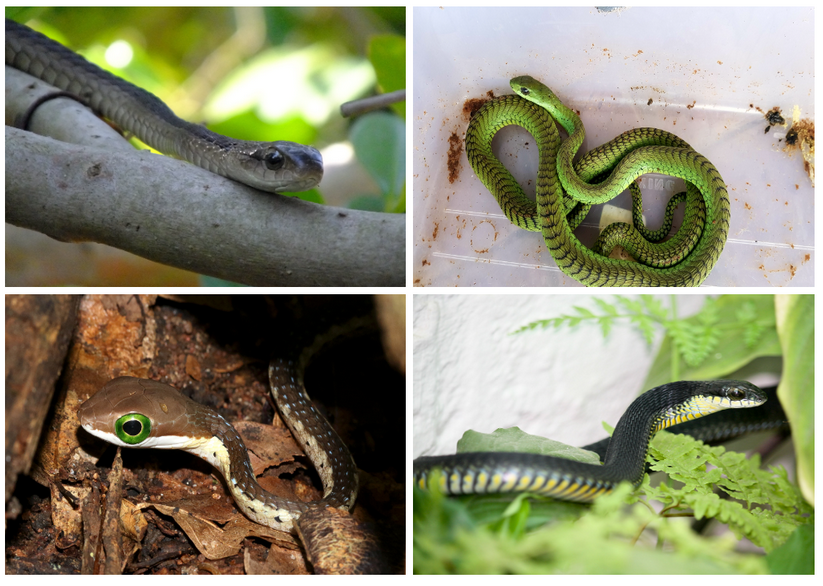
\includegraphics[width=0.59\columnwidth]{IntraClassVar}
  \caption{Four images of the Dispholidus Typus snake species with high visual deviation characterized by age and gender depicting an instance of high inter-class variance in the data set}
  \label{fig2_intraclass_var}
\end{figure}


\section{Related Work}

An investigation of the accuracy of five machine learning techniques — decision tree J48, nearest neighbors, k-nearest neighbors (k-NN), back-propagation neural network, and naive Bayes — for image-based snake species identification problem was performed in \cite{amir}. It revealed the efficacy of back-propagation neural networks which achieved a greater than 87\% classification accuracy. 

A Siamese network with three main components namely, twin network, similarity function and output neuron was proposed in \cite{abeysinghe} to classify the snake species. A pair of deep neural networks was proposed where one network extracts features from the test image while the other from a reference image. The features were compared using L1 distance similarity and the final output layer predicted the probability of the test image belonging to same class as the reference image.

Four different region-based convolution neural networks (R-CNN) architectures - Inception V2, MobileNet, ResNet and VGG16 were used in \cite{patel} for object detection and image recognition of 9 snake species of the Pseudalsophis genus. Among them, VGG16 and ResNet achieved the highest accuracy of 75\%.

A detailed quantitative comparative study between a computer vision algorithm trained to identify 45 species and human experts was performed in \cite{durso}. The algorithm used an EfficientNet based model, fine-tuned using preprocessed images to achieve an accuracy between 72 and 87\% depending on the test data set. The significant impact of geographic data in addition to visual information for snake species classification was also realized.

\section{Methodology}

A transfer learning method is adopted to classify the snake species using the data set of snake images and geographic location metadata provided by SnakeCLEF-2021 \cite{lifeclef2021, snakeclef2021}. The pre-trained Inception ResNet V2, a deep learning convolution neural network is used to extract image features. These features are concatenated with the categorical geographic features and finally classified using a gradient boost classifier.

\subsection{Preprocessing}

The input images were resized to $299\times299\times3$ using bi-linear interpolation. To counter the effect of irrelevant factors in the context of the required task such as variation in lighting conditions among the photographs, the images were linearly normalized to values between 0 and 1.

Scale and rotation transformations, along with contrast and saturation variations were performed to make the model more generic, immune to the impact of positional and orientation based features and prevent memorization by enhancing image diversity. RandAugment \cite{rand_augment} was used to augment the input images using the aforementioned transformations. RandAugment is parameterized by two values - the number of augmentation transformations to apply sequentially (N), and the magnitude for all the transformations (M). The values used in \cite{rand_augment} for the ResNet model i.e N=3 and M=4 were chosen. 

\subsection{Feature Extraction}

The Inception ResNet V2 model was used to perform feature extraction. The model is loaded with weights obtained from pre-training on the ImageNet data set. The fully connected output layer was excluded from the base model. A 2D average pooling layer is appended to produce the representation vector of the input image.

The pre-processed images are fed to the so constructed convolution neural network to produce a feature vector. We have obtained 1536 features for each input image from the output layer. This vector is then augmented with the geographic metadata, containing country and continent information, to perform the snake species classification.

\subsection{Gradient Boost Classifier}

A decision tree ensemble classifier is trained using the metadata about the geographic location of the photograph along with the image feature vector obtained form the Inception ResNet V2. Gradient boosting algorithm is used to train the classifier. The parameters of the classifier are tuned over several runs to improve classification results. 

Five-fold cross-validation is used to obtain a reliable evaluation of model performance for each configuration of parameters. The classifier is trained five times per run, each time selecting a different fold as the cross-validation set and training on the remaining four folds. The average of the performance parameters ( accuracy and F1 score ) over the five iterations is considered while tuning the parameters. Cross-entropy loss is used to monitor the model's convergence towards the objective in each fold. Early stopping is used to stop the boosting process if the loss starts to diverge.

\section{Implementation Details}

The training subset consisting of 347,406 images was split into five folds for cross-validation while training the classifier. Since the data-set had a long-tailed distribution across classes, stratified sampling was used to ensure a proportional split and ensure inclusion of images from each class.

The pre-processed images from the training and validation set are fed into the proposed deep learning convolution neural network model. The model produces feature-vectors of size 1536 for each image. 

The geographic location describing where the photographs were taken, specifically the continent and country, are encoded into numeric labels. This information is used as categorical features in classifier. For the images in which this data is unavailable, the features are encoded as 'nan'. The classifier imputes the missing values to the mode of the corresponding feature space. The representation vector consisting of 1538 features obtained for each image is used to train the decision tree ensemble classifiers by gradient boosting.

It was observed that learning rates higher than 0.05 lead to quicker divergence, suggesting the suitability of a slower learning rate using with more decision trees. Grid-search was performed by varying the learning rates in the range of 0.001 to 0.05 and the number of decision trees in the range 100 to 1000. Combinations having the least losses were chosen to further tune the tree-level parameters.

The maximum depth for the tree is left to be determined based on the training progress of the classifier and is not set strictly. This causes the depth to expand until the leaves are pure (has all samples belonging to the same class) or has reached the threshold of minimum number of samples required to split further. Due to the long-tailed distribution of the data set, some classes may require deeper branches to capture more information from the features. The potential over-fitting that may occur is controlled by tuning and setting an upper limit on the number of leaves by performing a grid search over values in range of 32 to 256.

Some other notable tree-level parameters tuned were sub-sampling rate and column-sampling rate. Sub-sampling rate determines the fraction of training samples that are randomly sampled per tree and was tuned between 0.6 and 1.0. Column-sampling rate, on the other hand, specifies the fraction of features used to fit each decision tree and was tuned between 0.5 and 0.9. Both these parameters help prevent over-fitting. They are maintained sufficiently above 0.1 to prevent under-fitting.

\section{Results}

The country and continent metadata, used as categorical features in the classifier had a significant impact on the classification. Without the categorical data, the testing accuracy of the best run was 40.16\%. This improved to 42.96\% when contextual data was encoded as categorical features. Country information has the highest impact while continent information also has a notable influence on the classification. Figure \ref{fig1_feature_imp}, depicts the relative importance of the 20 most significant features of the 1538 features used for classification. The feature importance values are normalized and scaled between 0 and 100 to realise the relative impacts. Features named as f1, f2, etc. denote features extracted from the convolution neural network.

\begin{figure}[!hbt]
  \centering
  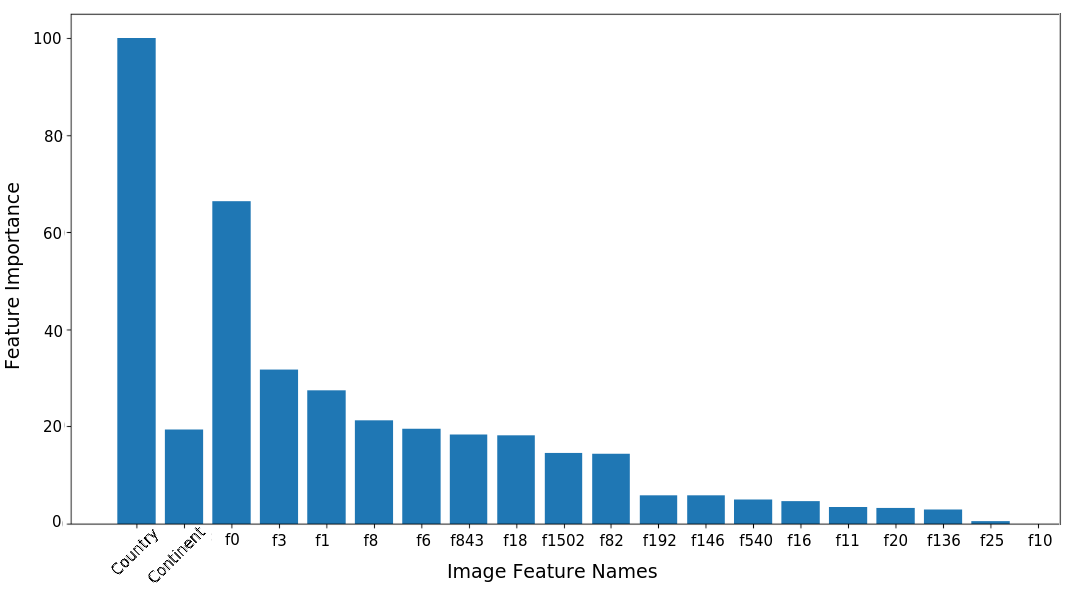
\includegraphics[width=1.0\columnwidth]{FeatureImp}
  \caption{Relative importance on a scale of 0-100 of the 20 most impactful features used to train the classifier. The first two bars represent feature importance of \textbf{country} and \textbf{continent} respectively}
  \label{fig1_feature_imp}
\end{figure}

Through parameter tuning, the classifier's performance was improved over several runs. The F1-scores macro-averaged across the countries and macro-averaged over all classes were the prescribed the metrics \cite{snakeclef2021}. Eight best runs were selected based on the prescribed metrics evaluated on the prescribed validation set. The metrics are evaluated as an average over the five iterations (for 5-fold cross validation) performed in each run. We have achieved a training accuracy of 71.32\%, validation accuracy of 44.16\% and a testing accuracy of 42.96\% on the best run. The results are summarized in Tables \ref{performance_table_val} and \ref{performance_table_test} below:

\begin{center}
    \begin{table}[!hbt]
        \caption{Prediction metrics of the five best runs on the validation set}
        \begin{tabular}{|c|c|c|c|}
            \toprule
             Run & F1-Score (Country) & F1-Score (Overall) & Accuracy \\
             \midrule  
             1 & 0.455 & 0.456 & 0.531 \\ 
             2 & 0.482 & 0.469 & 0.554 \\  
             3 & 0.509 & 0.481 & 0.569 \\   
             4 & 0.522 & 0.488 & 0.583 \\ 
             5 & 0.536 & 0.497 & 0.622 \\
             \bottomrule
        \end{tabular}
        \label{performance_table_val}
    \end{table}
\end{center}

\begin{center}
    \begin{table}[!hbt]
        \caption{Prediction metrics of the five best runs on the test set}
        \begin{tabular}{|c|c|c|c|}
            \toprule
             Run & F1-Score (Country) & F1-Score (Overall) & Accuracy \\
             \midrule
             1 & 0.246 & 0.164 & 0.428 \\
             2 & 0.247 & 0.166 & 0.430 \\  
             3 & 0.249 & 0.159 & 0.428 \\   
             4 & 0.249 & 0.162 & 0.432 \\ 
             5 & 0.252 & 0.162 & 0.432 \\
             \bottomrule
        \end{tabular}
        \label{performance_table_test}
    \end{table}
\end{center}

\section{Conclusion and Future Work}

The results depict the positive impact of integrating contextual country and continent data for snake species classification. Introducing more contextual data such as population counts of various species by region as class-wise probability priors \cite{wang}, climate information such as temperature and humidity, etc. may contribute to better classification results. 

Due to unavailability of sufficient computational resources during the SnakeCLEF-2021 contest period, the results were submitted before complete convergence of the classifier's training process. Post the deadline, significant improvements in classification accuracy were observed even with a slight increase in the number of iterations applied to train the gradient boost classifier. This suggests that the transfer learning approach adopted here is promising and further parameter tuning and complete training can greatly improve the model performance.

Further efforts to experiment with input image resolutions and alternative pre-trained weights \cite{picek} as well as including custom training layers to the frozen base model before extracting features \cite{zhong} can contribute to the classification performance.

\begin{acknowledgments}
  Thanks to the Machine Learning Research Group (MLRG), Deptartment of Computer Science and Engineering, Sri Sivasubramaniya Nadar College of Engineering, Chennai, India
  ( \url{https://www.ssn.edu.in/} ) for providing the GPU resources to implement the model
\end{acknowledgments}

\bibliography{references}  
\end{document}
%% End of file
